%!TEX root = ../main.tex
\chapter{Validation} % (fold)
\label{cha:validation}

\section{Presentation of the toy problems}

Two toy problems are set up to demonstrate
the capabilities and the limitations of the harmonic
balance approach, either mono-frequential or multi-frequential.




\section{Channel flow}
\label{sec:channel-flow}

\subsection{Test case description}
% presentation of the channel case
A channel configuration is set up to study the properties of the
proposed HB method and the above algorithms for non-uniform time
sampling.  It is a 2D channel of length $L_x = 100$~m in the axial
direction and $L_z = 1$~m in the transverse one.  The boundary
conditions are: (i)~an injection condition for the inlet,
(ii)~symmetric conditions for the upper and lower bounds as the flow
is assumed to be symmetric in the transverse direction, and (iii)~a
fluctuating pressure imposed at the outlet:
\begin{equation}
  P_{outlet}(t) = P_m \cdot \left[1 + A_1 \cdot \sin(2 \pi f_1 t) +
    A_2 \cdot \sin(2 \pi f_2 t) \right],
  \label{eq:outlet_canal}
\end{equation}
where $P_m$ is the temporal average static pressure, $A_n$ the
amplitude of the $n$\textsuperscript{th} mode and $f_n$ its
frequency. The mean outlet pressure $P_m$ is set to $60\%$ of the
inlet total pressure $P_{i0} = 101,325$~Pa.

Pressure waves travel within the flow with the velocity $u + c$ and $u
- c$, where $u$ denotes the local flow velocity and $c$ the sound
velocity. Since the pressure waves are generated at the outlet, only
the $u-c$ waves are visible, resulting in pressure waves propagating
upstream of the channel, which are damped by the effect of
viscosity. Figure~\ref{fig:canal_principle} shows a schematic diagram
of the channel case, illustrating the propagation and attenuation of
the pressure waves.
\begin{figure}[htb]
  \centering
  \includegraphics*[width=0.6\textwidth]{CANAL2_PRINCIPLE.eps}
  \caption{Schematic diagram of the channel case.}
  \label{fig:canal_principle}
\end{figure}

% mesh presentation
The mesh consists of 997~points along the axial direction and 9 in the
transverse one, which amounts to almost equal spacings in both
directions.


This configuration is turbulent as the Reynolds number based on the
inlet flow velocity and the axial length of the channel is about $R_e
\approx 2.0 \times 10^9$.  Turbulence is modeled using the
one-equation model of Spalart and Allmaras~\cite{Spalart1992}, and the
third-order upwind Roe scheme~\cite{Roe1981} is used to compute the
convective fluxes.

\subsection{Convergence sensibility analysis}

As mentioned previously, the condition number is of great importance
for the convergence of the proposed HB method. To highlight this
feature, the presented channel case is computed with a single
frequency at the outlet: $f_1 = 3$~Hz with an amplitude $A_1 = 0.05$
for the first case and $A_1=0.01$ for the second one, the second
frequency having a zero amplitude: $A_2= 0$.  Two frequencies are
specified for the HB computation: $f_1$ and its first harmonic
$2f_1$. The time levels are chosen to reach varying condition numbers
such that $1 \leq \kappa (A) \leq 3.43$.  Since the input frequencies of the HB
computation are harmonically related, the minimal conditioning
$\kappa(A) = 1$ is obtained with evenly spaced time levels.  The OPT
algorithm is modified by subtracting the targeted conditioning to the
objective function, so that the different condition numbers can be
reached.  The distribution of the time levels for each condition
number is shown in Fig.~\ref{fig:canal2_distribution_tlv}.  The time
levels deviate from the evenly spaced solution as the condition number
grows.
\begin{figure}[htb]
  \centering \subfigure[Relative to period
  $1/f_1$]{\includegraphics[width=.45\textwidth]{CANAL2_RESIDUAL_VS_CONDITIONNING_TLV_REPARTITION_F1.eps}}
  \quad \subfigure[Relative to period
  $1/2f_1$]{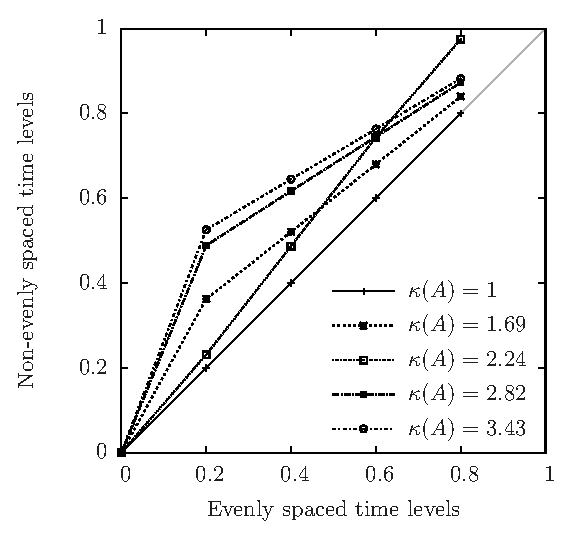
\includegraphics[width=.45\textwidth]{CANAL2_RESIDUAL_VS_CONDITIONNING_TLV_REPARTITION_F2.eps}}
  \caption{Distribution of the time levels on each frequency periods.}
  \label{fig:canal2_distribution_tlv}
\end{figure}
The results in Fig.~\ref{fig:canal_residual_vs_conditionning} show that
for a condition number $\kappa (A) \geq 3.43$ and wave input amplitude
$A_1 = 0.05$, the computation diverges. However, the computations with
the same condition numbers but a smaller input amplitude $A_1 = 0.01$
converge. In fact, the condition number amplifies the errors made
during the iterative process. When the input waves have a smaller
amplitude, the iterative errors are slighter, hence the convergence as
explained \S~\ref{sec:condition_number}.
\begin{figure}[htb]
  \centering \subfigure[$A_1 =
  0.01$]{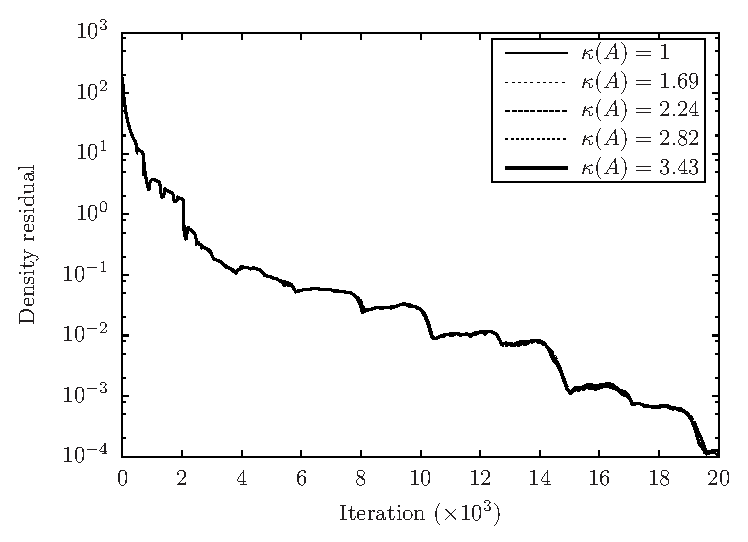
\includegraphics[width=.45\textwidth]{CANAL2_RESIDUAL_VS_CONDITIONNING_AMP001.eps}}
  \quad
  \subfigure[$A_1=0.05$]{\includegraphics[width=.45\textwidth]{CANAL2_RESIDUAL_VS_CONDITIONNING_AMP005.eps}}
  \caption{Relation between the condition number $\kappa (A)$ and the
    convergence of the solution.}
  \label{fig:canal_residual_vs_conditionning}
\end{figure}


\subsection{Validation of the multi-frequency HB method}

To validate the proposed HB method, two non-harmonically related
frequencies are chosen as input for the outlet boundary condition:
$f_1 = 3$~Hz and $f_2 = 17$~Hz.

A classical time-marching scheme is taken for comparison, namely the
Dual Time Stepping scheme (DTS~\cite{Jameson1991}).  The DTS method is
a 2\textsuperscript{nd}-order implicit time-marching scheme.
Convergence in time discretization is obtained after 20~periods using
160~instants per almost-period. Since the frequencies are integers and
coprime, the period is $T=1$~s.  Iterative convergence for the
inner loop is considered achieved when the normalized residuals drop
by $10^{-2}$ within a maximum of 50~sub-iterations.

The results obtained with the DTS scheme are compared to the HB
results for pressure waves amplitudes of $A = A_1 = A_2 = 0.001$.  The
transient of the DTS computation is shown
Fig.~\ref{fig:canal2_transient}, illustrating the wave propagation
with a slight attenuation of the high-frequency waves.
%The waves propagating upstream vanishing with the effect of viscosity
%are highlighted.
\begin{figure}[htbp]
  \centering
  \includegraphics*[width=.7\linewidth]{CANAL2_TRANSIENT.eps}
  \caption{DTS computation: transient propagation of the pressure waves.}
  \label{fig:canal2_transient}
\end{figure}


%Firstly, the DTS results are verified to yield a
%time-converged solution. =>deja dit plus haut !
The results are analyzed for frequencies $1<f< 40~\textrm{Hz}$ and the
dominant frequencies (the one that have the highest amplitudes) are
set for the HB computation.  To do so, pressure signals are probed
upstream, in the middle and downstream of the channel at
$x=[25~\textrm{m}, 50~\textrm{m}, 75~\textrm{m}]$ and $z=0.5$~m
respectively.  The spectrum of the aforementioned unsteady pressure
signals, obtained with a Fourier Transform, are plotted
Fig.~\ref{fig:canal2_dts_fft}.  The labeled frequencies are the
dominant ones, as for each probe, these have a high amplitude. They
are thus selected for the HB computation.  For such frequencies, the
OPT algorithm gives a set of time levels leading to a condition number
of~1.4.
\begin{figure}[htb]
  \centering
  \includegraphics*[width=.6\linewidth]{CANAL2_PROBE_POSITION.eps}

  \vspace{1em}

  \includegraphics*[width=.6\linewidth]{CANAL2_DTS_FFT.eps}
  \caption{Spectrum of pressure signals.}
  \label{fig:canal2_dts_fft}
\end{figure}

A Discrete Fourier Transform is computed at several axis positions,
resulting in the spatial evolution of the different harmonics, which
is used for the comparison of the HB and DTS approaches, in the middle
of the canal ($z = 0.5$~m).  In
Fig.~\ref{fig:canal2_validation_hbt_gear_amp_vs_axis}, the results are
plotted for the frequencies that have been set for the HB computation.
The overall agreement is fair.  Some local discrepancies can be
observed upstream for frequencies $f_2 + 3f_1$, $f_2 - f_1$ and $f_2 -
2f_1$. These are caused by aliasing
 but they are minimal regarding the temporal evolution, as
shown in Fig.~\ref{fig:canal2_validation_hbt_gear_time_ev}, where the
time evolution of pressure signals is extracted at all probes.  The
difference between the HB and the DTS method is negligible, proving
that the proposed HB method is able to reproduce the unsteady
almost-periodic phenomena.
\begin{figure}[htbp]
  \centering
  \includegraphics*[width=.7\linewidth]{CANAL2_VALIDATION_HBT_GEAR_AMP_VS_AXIS.eps}
  \caption{Spatial evolution of the amplitude of the dominant
    frequencies in the channel, for $f_1 = 3$~Hz and $f_2 = 17$~Hz.}
  \label{fig:canal2_validation_hbt_gear_amp_vs_axis}
\end{figure}

\begin{figure}[htb]
  \centering 
  \subfigure[Probe
  1]{\includegraphics[width=.45\textwidth]{CANAL2_VALIDATION_HBT_GEAR_TIME_EV_PROBE_1.eps}}
   \quad\subfigure[Probe
   2]{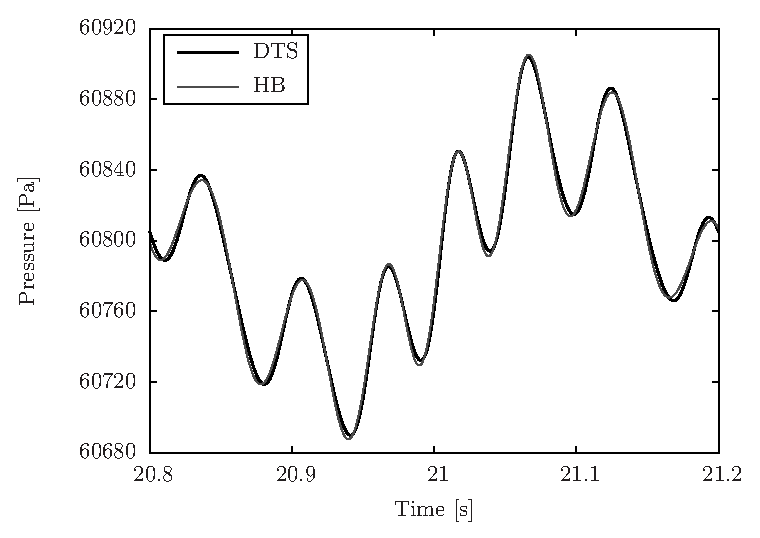
\includegraphics[width=.45\textwidth]{CANAL2_VALIDATION_HBT_GEAR_TIME_EV_PROBE_2.eps}}
   \subfigure[Probe
   3]{\includegraphics[width=.45\textwidth]{CANAL2_VALIDATION_HBT_GEAR_TIME_EV_PROBE_3.eps}}
  \caption{Unsteady pressure signals at different axial positions.}
  \label{fig:canal2_validation_hbt_gear_time_ev}
\end{figure}

The goal of this section was not to show significant CPU savings but
rather the capacity of the present HB method to capture an
almost-periodic flow on a model problem.  It is now applied to a more
complex configuration, namely a turbomachinery element, where its
computational efficiency is also emphasized.






\section{Convection equation solver}




% chapter validation (end)